\documentclass[letterpaper,10pt,conference]{ieeeconf}
\IEEEoverridecommandlockouts
\overrideIEEEmargins
\usepackage{graphicx}
\usepackage{adjustbox}
\usepackage{amsmath,amssymb}
\usepackage{booktabs}
\usepackage{multirow}
\usepackage{array}
\usepackage{tabularx}
\usepackage{tikz}
\usetikzlibrary{arrows.meta,positioning}
\usepackage{pgfplots}
\pgfplotsset{compat=1.18}
\usepackage{xcolor}
\usepackage{url}
\usepackage{float}
\usepackage{placeins}
\usepackage{capt-of}
\definecolor{PoseColor}{RGB}{35,100,180}
\definecolor{MoveColor}{RGB}{180,80,40}
\definecolor{PathColor}{RGB}{60,130,80}
\definecolor{AvailNative}{RGB}{30,140,70}
\definecolor{AvailRemat}{RGB}{120,60,160}
\definecolor{AvailNone}{RGB}{200,40,40}
\newcommand{\posecolor}[1]{\texttt{\textbf{\textcolor{PoseColor}{#1}}}}
\newcommand{\movecolor}[1]{\texttt{\textbf{\textcolor{MoveColor}{#1}}}}
\newcommand{\pathcolor}[1]{\texttt{\textbf{\textcolor{PathColor}{#1}}}}
% Table~I feasibility: native / rematerialize / unavailable
\newcommand{\availok}{\textcolor{AvailNative}{\checkmark}}
\newcommand{\availrem}{\textcolor{AvailRemat}{$\triangle$}}
\newcommand{\availno}{\textcolor{AvailNone}{$\times$}}
% Table color map: black = match Core; red = mismatch; blue = rematerialized channel
\newcommand{\semok}[1]{#1}
\newcommand{\sembad}[1]{\textcolor{red!70!black}{\textbf{#1}}}
\newcommand{\semadapt}[1]{\textcolor{blue!65!black}{\textbf{#1}}}
\newcommand{\jointseq}{Joint-Space Sequence}
\newcommand{\cartseq}{Cartesian-Space Sequence}
\newcommand{\method}{Motion Program}
\newcommand{\methodfull}{Symbolic Motion Program}
\newcommand{\traj}{Selective Cartesian}
\newcommand{\trajfull}{Selective Cartesian}
\newcommand{\TBD}[1]{\textcolor{red!70!black}{\textbf{#1}}}

% ---------------------------------------------------------------------------
% CENTRAL STANCE (fixed before revising the text):
%   Embodied agents are expressive whether or not they were designed to be;
%   because humans read meaning across radically different bodies, the failure
%   of gesture generation off the human body reflects a generator that imitates
%   human surface form without understanding which evidence carries meaning.
% ---------------------------------------------------------------------------

% --- float placement: one full-width plus one column float is typical
\setcounter{topnumber}{2}
\setcounter{bottomnumber}{1}
\setcounter{totalnumber}{2}
\setcounter{dbltopnumber}{2}
\renewcommand{\topfraction}{0.70}
\renewcommand{\bottomfraction}{0.55}
\renewcommand{\dbltopfraction}{0.9}
\renewcommand{\textfraction}{0.08}
\renewcommand{\floatpagefraction}{0.7}
\renewcommand{\dblfloatpagefraction}{0.55}

\title{One Grammar, Many Robots: LLM-Driven\\Automatic Gesture Generation Across Embodiments}
\author{Anonymous Authors\thanks{Anonymous submission. Identifying links are omitted for double-anonymous review.}}

\begin{document}
\maketitle
\thispagestyle{empty}
\pagestyle{empty}

\begin{abstract}
Embodied agents are expressive whether or not they were designed to be. People read intent from the motion of other people, animals, and even moving shapes, and they read it through carriers as different as a hand and a tail. A robot's motion will therefore be interpreted; what remains open is whether it is interpreted as intended. Current gesture generation largely imitates the surface form of human gestures without representing which evidence makes them recognizable, and we argue that this imitation without understanding is why generation breaks once the body is no longer human. We identify \emph{orientation}, \emph{body-relative location}, and \emph{movement} as recognition-critical attributes and describe transfer to a new body as preserving, carrier-transferring, or rematerializing them. As an intermediate interface until models can reason about their own morphology, \textit{\methodfull{}s} (\method{}s) expose these attributes as executable \texttt{pose}, \texttt{movement}, and \texttt{path} primitives. Even on human-like bodies that provide every necessary carrier, LLM-authored programs are recognized at only $63.3\%$ on Unitree~G1 and $60.0\%$ on Tiago on a 30-cue screen, against $96.7\%$ and $93.3\%$ for human-authored programs, and at $54.4\%$ on a harder 90-cue G1 4AFC ($25\%$ chance); attribute-level analysis traces the gap to incorrect orientation, placement, and stroke. On IIWA, Stretch, Roomba, and three synthetic bodies, generation draws on a narrower repertoire, and distinct meanings collapse onto the same remaining stroke. We read these gaps as evidence about how gestures are generated, not as a benchmark ceiling.
\end{abstract}

\section{Introduction}
Robot motion is interpreted whether or not it was designed to communicate. We take this as the starting point of the paper: embodied agents are expressive whether or not they were designed to be, so the question for a robot is not \emph{whether} its motion carries meaning, but whether it carries the meaning that was intended.

This stance rests on more than a tendency to anthropomorphize moving things. Humans infer intent, emotion, and even personality from agents far beyond human adults, down to geometric shapes in motion~\cite{heider1944apparent} and a handful of moving points of light~\cite{johansson1973biological}. Darwin already treated bodily expression as continuous across species~\cite{darwin1872expression}, and ethology describes how ordinary movements are \emph{ritualized} into displays whose function is to be read by another animal~\cite{tinbergen1952derived,maynardsmith2003signals}. Comparative work on ostension shows that the manner of a movement can itself mark it as communicative rather than instrumental~\cite{tomasello2008origins,moore2016meaning}, and legible robot motion builds on the same capacity to infer intent from a trajectory~\cite{dragan2013legibility}. None of this is tied to a human skeleton: people can tell what a dog's wagging tail signals~\cite{quaranta2007tail}, and they understand a gesture made with a prosthetic limb that no biological hand produced. Observers read meaning from the evidence a motion carries, not from the anatomy that carries it.

\begin{figure}[t]
\centering
\begin{minipage}[t]{0.47\columnwidth}
\centering
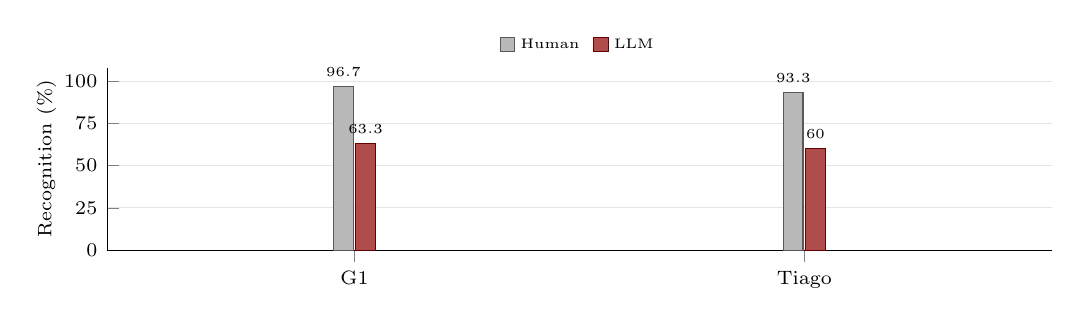
\begin{tikzpicture}
\begin{axis}[
  ybar=1pt, bar width=7pt,
  width=1.12\linewidth, height=3.9cm,
  ymin=0, ymax=108, ytick={0,25,50,75,100},
  ylabel={Recognition (\%)}, ylabel style={font=\scriptsize, yshift=-4pt},
  symbolic x coords={G1,Tiago}, xtick=data, enlarge x limits=0.55,
  tick label style={font=\scriptsize},
  nodes near coords, every node near coord/.append style={font=\tiny, /pgf/number format/fixed, /pgf/number format/precision=1},
  legend image code/.code={\draw[#1] (0cm,-0.08cm) rectangle (0.18cm,0.1cm);},
  legend style={at={(0.5,1.02)}, anchor=south, font=\tiny, draw=none, fill=none, legend columns=2, /tikz/every even column/.append style={column sep=3pt}}, axis lines*=left, ymajorgrids, grid style={gray!20},
]
\addplot[fill=gray!55, draw=gray!70!black] coordinates {(G1,96.7) (Tiago,93.3)};
\addplot[fill=red!55!black!70, draw=red!40!black] coordinates {(G1,63.3) (Tiago,60.0)};
\legend{Human, LLM}
\end{axis}
\end{tikzpicture}\\[-1pt]
{\scriptsize (a) Same carriers, different author}
\end{minipage}\hfill
\begin{minipage}[t]{0.51\columnwidth}
\centering
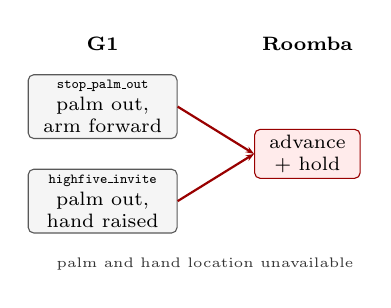
\begin{tikzpicture}[
  cue/.style={draw=gray!70!black, rounded corners=2pt, align=center, font=\scriptsize, inner sep=2pt, text width=1.75cm, fill=gray!8},
  col/.style={font=\scriptsize\bfseries},
  arr/.style={-{Stealth[length=3pt]}, thick, red!60!black}]
\node[col] (h) at (0,1.65) {G1};
\node[col] (r) at (2.6,1.65) {Roomba};
\node[cue] (s) at (0,0.85) {{\tiny\texttt{stop\_palm\_out}}\\ palm out, arm forward};
\node[cue] (f) at (0,-0.35) {{\tiny\texttt{highfive\_invite}}\\ palm out, hand raised};
\node[cue, fill=red!8, draw=red!60!black, text width=1.2cm] (c) at (2.6,0.25) {advance\\ $+$ hold};
\draw[arr] (s.east) -- (c.west);
\draw[arr] (f.east) -- (c.west);
\node[font=\tiny, text=gray!40!black, align=center] at (1.3,-1.15) {palm and hand location unavailable};
\end{tikzpicture}\\[2pt]
{\scriptsize (b) Off the human body: contrast collapse}
\end{minipage}
\caption{\textbf{Imitation without understanding, and its collapse off the human body.} (a) On human-like bodies that provide every carrier a gesture needs, LLM-authored Motion Programs are recognized far less often than human-authored ones (30-cue screen). (b) Once palm orientation and hand location are unavailable, cues that differ only in those attributes collapse onto the same base motion on Roomba (Sec.~\ref{sec:results-constrained}). Panel (b) schematizes a qualitative observation; constrained-body recognition rates are not yet measured.}
\label{fig:teaser}
\end{figure}

Robot gesture generation has rarely been built on this view. Most research on expressive robot motion asks how a robot conveys affect, personality, or internal state through global motion qualities~\cite{zhou2017timing,knight2014xytheta,knight2016laban}, or how a human-like body produces natural co-speech movement~\cite{kucherenko2020gesticulator,yoon2020trimodal,liu2022beat}. Such generators learn what a gesture \emph{looks like} on a human body rather than which evidence makes it recognizable---\emph{imitation without understanding}. Even on human-like bodies this imitation is incomplete: orientation, placement, and stroke are frequently wrong (Fig.~\ref{fig:teaser}a). Once the body departs from the human template, there is no longer a form to copy, and the generator must decide which carrier and which stroke will keep the meaning intact; performance then collapses (Fig.~\ref{fig:teaser}b). The results in this paper should be read in that light: the gap between human- and LLM-authored gestures, and its widening off the human body, are evidence about what current generation does not understand, not a benchmark gap to be closed by a better renderer.

Two coupled properties of gesture make the problem hard. First, gesture realization and recognition involve an inherently many-to-many mapping between meaning and action. A greeting wave, for example, can be realized through innumerable variations in hand position, arm configuration, and movement, while some realizations remain more typical or canonical than others. Second, on non-humanoid bodies the mapping between a gesture and its carrier is \textit{not strict}: the availability of a particular body part (a head for nodding) is not always essential to the gesture, whose repeated stroke can be carried by another body part or reformulated on a mobile base. This transfer is not simple anatomical matching: some communicative attributes can be realized through seemingly incompatible body parts, while others cannot be recovered once the relevant morphological structure disappears. We therefore hold discrete communicative meanings fixed---such as beckoning, depicting a flying bird, or inviting a high five---and vary the body.

To describe what must survive, we identify three recognition-critical attributes---\textit{Orientation}, \textit{Location}, and \textit{Movement}---that contribute to canonical realizations of a given cue. For a greeting wave, raising the hand (\textit{Location}), presenting the palm (\textit{Orientation}), and producing lateral movement (\textit{Movement}) each contribute to a canonical motion, while variations that omit or alter some of these attributes may still preserve the intended meaning. This flexibility is what makes transfer across morphologies possible, and we characterize it through three realization strategies: preservation, carrier transfer, and rematerialization.

Understanding which attributes matter does not by itself yield a model that can reason about an unfamiliar body. As an intermediate step, we introduce \textit{\methodfull{}s}, a symbolic interface that makes the attributes explicit. Humans and LLMs author gestures in the same \texttt{pose}/\texttt{movement}/\texttt{path} representation, which is compiled deterministically across robot bodies and remains editable and diagnosable at the attribute level. The representation is not the goal; it is a stopgap that lets us generate gestures today and localize what automatic authoring misses. Our experiments reveal a substantial recognition gap between human- and LLM-authored programs on G1 and Tiago (human-authored $96.7\%$ and $93.3\%$ vs LLM-authored $63.3\%$ and $60.0\%$), with recurring attribute errors such as incorrect hand orientation for air quotes. On IIWA, Stretch, and Roomba, generation relies on a narrower repertoire of transfers and substitutes: some meanings survive rematerialization onto a kinematic chain, mast, or mobile base, while others collapse together once palms, head motion, or bilateral structure disappear. Three synthetic morphologies extend the test to novel combinations of carriers. Our contributions are:
\begin{enumerate}
\setlength{\itemsep}{0.1em}
\item \textbf{A perceptual formulation of cross-embodiment gesture}: discrete meanings are described through orientation, body-relative location, and movement, and their transfer as preservation, carrier transfer, or rematerialization.
\item \textbf{An executable, editable intermediate interface}: Motion Programs let humans and LLMs author the same representation and compile it across bodies while models cannot yet reason about morphology directly.
\item \textbf{Evidence of imitation without understanding}: humanoid experiments and constrained-body cases show where generated gestures preserve, rematerialize, augment, distort, or lose communicative evidence.
\end{enumerate}

\section{Related Work}
Prior work on robot gesture largely treats the human skeleton as a constant and asks whether motion on it is natural, appropriate, or expressive; we instead hold meaning constant and let the body vary.

\subsection{Expressive Robot Motion Generation}
Communicative robot behavior has been authored through multimodal behavior languages and robot-specific gesture systems~\cite{kopp2006bml,salem2012gesture,chidambaram2012gesture} or learned from paired speech and human motion~\cite{kucherenko2020gesticulator,yoon2020trimodal,liu2022beat}.
These approaches model semantics, affect, style, and speech synchrony, but usually retain a stable human-like skeleton and ask whether the resulting motion is natural or socially appropriate.
They therefore address variation within an embodiment more directly than preservation of a discrete meaning across embodiments.
Timing, energy, and Laban-derived qualities alter perceived confidence, naturalness, and state on heads, mobile bases, and other low-degree-of-freedom platforms~\cite{zhou2017timing,knight2014xytheta,knight2016laban}.
This work establishes that non-humanoid motion can be socially legible, but often studies an affective dimension or a platform-specific repertoire rather than a shared inventory of discrete gestures.
Our study follows one such inventory from humanoids to a single arm, an extensible mobile manipulator, a planar base, and unfamiliar synthetic bodies.

\subsection{Motion Generation with Large Language Models}
Language models generate robot motion at several levels: they can emit code that invokes skills~\cite{liang2023cap}, construct spatial objectives or value maps that guide control~\cite{huang2023voxposer}, select or parameterize learned motion primitives~\cite{dai2026lmp}, and generate or retrieve expressive animations from a prompted repertoire~\cite{mahadevan2024generative}.
Across these systems, reliability is sought through structured APIs, few-shot demonstrations, executable constraints, objective construction, or verification and correction around the model output.
Most optimize task completion or assume a predefined skill library.
For gesture, however, physical execution is not the endpoint: the motion succeeds only when an observer recovers its intended meaning.
Our distinction is therefore representational: Motion Programs expose recognition-critical attributes as editable primitives, allowing the same automatic authoring pipeline to be retained across robots while the renderer changes how those attributes are physically realized.

\section{Gesture Generation Framework}
\label{sec:gesture}

\subsection{Gesture: Meaning and Action Mapping}

Gesture generation maps a \emph{meaning space} $\mathcal{G}$ (e.g., nodding yes, stopping, beckoning, or depicting a flying bird) to an \emph{action space} $\mathcal{A}(M)$ shaped by robot morphology $M$. For example, a Roomba realizes motion primarily through changes in $x$, $y$, and $\theta$, whereas a humanoid has many articulated carriers. Within each action space, a meaning can admit infinitely many continuous realizations, but not all variations contribute equally to recognition. We suggest that some attributes are \emph{recognition-critical}: changing them can weaken the evidence for the intended cue $G$ and shift interpretation toward plausible alternatives $G'$. For example, reversing the palm orientation in a \texttt{stop} gesture can make the motion resemble looking into a hand mirror.

\paragraph{Why non-humanoid bodies matter}
A non-humanoid $\mathcal{A}(M)$ is not only an architectural or kinematic challenge. Humans already read intent through radically different carriers---a wagging tail, a prosthetic limb, a moving shape (Sec.~I)---so when a meaning fails to come across on a single arm or a Roomba, the bottleneck need not lie in human perception. It may instead lie on the generation side: a generator that has learned only the surface form of human gestures does not know how to use an unfamiliar body to carry the same evidence. Separating these two explanations requires describing a gesture by the evidence it carries rather than by the body parts that usually produce it.

\subsection{Recognition-Critical Attributes}
\label{sec3.2}
In Figure~\ref{fig:critical-signatures}, we identify three attributes that commonly contribute to gesture recognition, with their relative importance varying across gesture cues. This formulation follows the category structure of \textit{family resemblance}~\cite{rosch1975family}, in which category members share overlapping features without requiring a single set of necessary and sufficient conditions, making some members more typical than others (e.g., $\operatorname{typ}(\text{robin}\mid\text{bird}) > \operatorname{typ}(\text{penguin}\mid\text{bird})$): individual attributes can make a realization more typical without every attribute being necessary.

\begin{figure}[t]
\centering
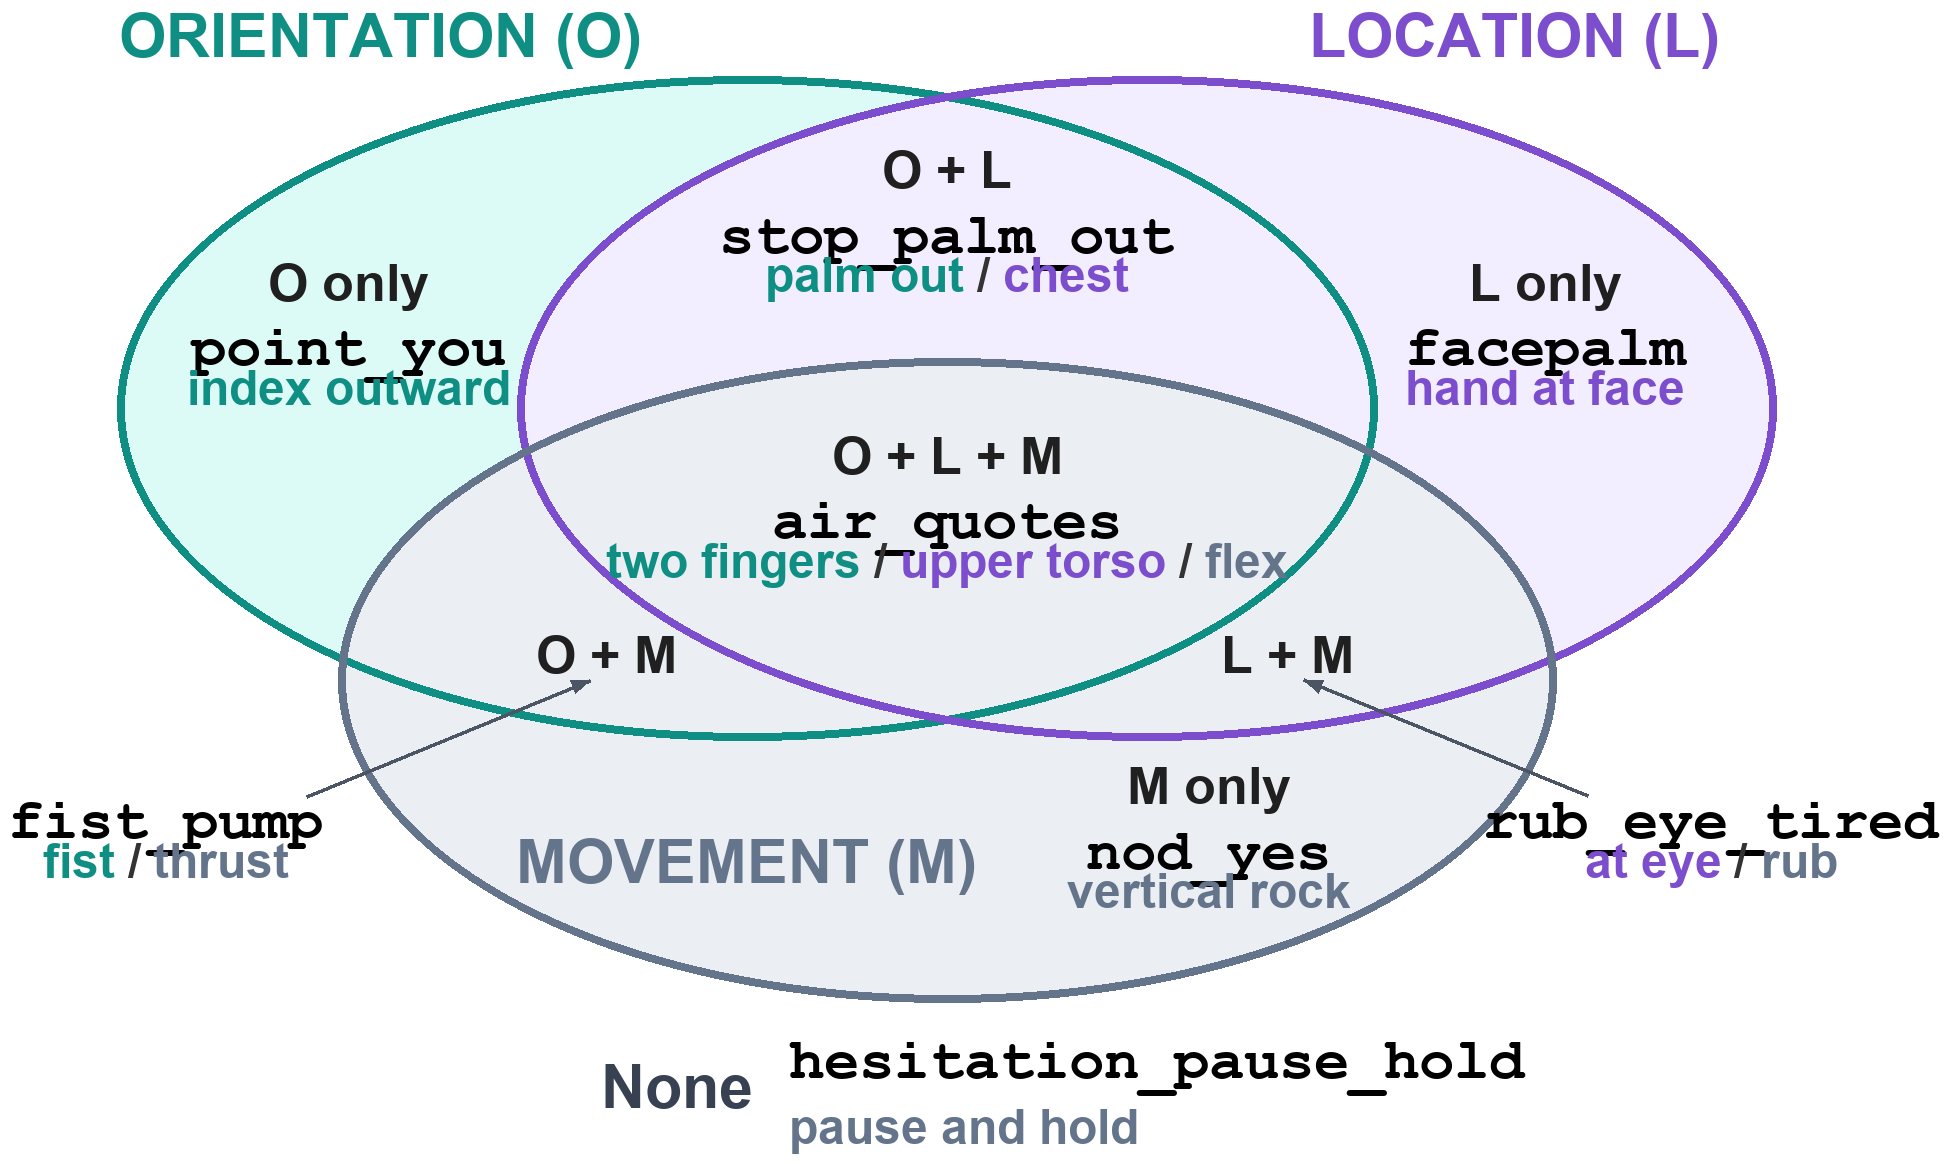
\includegraphics[width=\columnwidth]{figures/figure_critical_signature_venn.png}
\caption{We characterize gestures across morphologies through family resemblance: attributes such as \textit{Orientation}, \textit{Location}, and \textit{Movement} contribute with varying importance to the recognition of different gesture cues.}
\label{fig:critical-signatures}
\end{figure}

\paragraph{Orientation}
\textit{Orientation} describes where a recognition-relevant carrier---such as the head, hand, foot, torso, or end effector---is directed. The relevant carrier therefore depends on the robot morphology. Although orientation is physically continuous, we argue that many communicative distinctions can be captured by a small set of discrete relations: \textit{front}, \textit{back}, \textit{in}, \textit{out}, \textit{up}, and \textit{down}. For example, \texttt{point\_you} should orient its pointing carrier toward the addressee in \textit{front}; \texttt{stop\_palm\_out} presents the palm toward \textit{front} while directing the fingertips \textit{up}.

\paragraph{Location}
\textit{Location} describes where the relevant carrier lies relative to the body or environment. Location is naturally continuous and can require different spatial resolutions across cues, for example, in \texttt{rub\_eye} an incorrect $z$ coordinate can move the end effector from the eye to the forehead or nose, changing the intended interpretation. Therefore, continuous $(x,y,z)$ locations are needed to specify precise cue realization.

\paragraph{Movement}
\textit{Movement} describes how a carrier changes over time, including its axis, direction (sign), extent, speed, and repetition. Among these, axis and sign often provide particularly strong recognition evidence. A nod requires repeated motion along the \textit{vertical} ($z$) axis, whereas a head shake requires \textit{lateral} ($y$) oscillation. Thus, movement captures temporal structure that cannot be specified by pose alone.

\subsection{Transfer Across Morphologies}
\label{sec3.3}
The transfer taxonomy below is the mechanical counterpart of the perceptual claim above. If observers read evidence rather than anatomy, a gesture should survive a change of body whenever its evidence does---on the original carrier, on a different carrier, or in reformulated form---and fail only when that evidence is lost or distorted.

\paragraph{Carrier availability}
Transferring a gesture changes which carriers and attributes are physically available. Let $\mathcal{C}=\{O,L,M\}$ denote orientation, body-relative location, and movement, and let $\mathcal{H}(B)$ denote the independently usable realizations of $\mathcal{C}$ available on body $B$ (Table~\ref{tab:availability}). Movement structure is often comparatively portable: an axis, direction, or repetition pattern can be reconstructed with other body parts. Orientation may instead need to migrate to another carrier when the original one does not exist, while location is particularly morphology-dependent because body-relative landmarks and reachable regions change with embodiment.

\begin{table}[t]
\centering
\scriptsize
\setlength{\tabcolsep}{3pt}
\renewcommand{\arraystretch}{1.1}
\begin{tabularx}{\columnwidth}{@{}l>{$}l<{$}>{\raggedright\arraybackslash}X@{}}
\toprule
\textbf{Body} & \mathcal{H}(B) & \textbf{Carrier structure} \\
\midrule
G1 & \{O_{\rm palm/head},L_{\rm ee/head},M_{\rm art}\} & Full humanoid reference: articulated hands, two arms, head, torso. \\
Tiago & \{O_{\rm grip/head},L_{\rm ee/head},M_{\rm art/base}\} & Bilateral upper body and head; parallel grippers constrain palm orientation; base adds movement. \\
IIWA & \{O_{\rm grip/chain},L_{\rm ee},M_{\rm joint/ee}\} & Single arm; all evidence coupled to one kinematic chain. \\
Stretch & \{O_{\rm grip/base},L_{\rm mast/ee},M_{\rm joint/base}\} & Gripper, telescoping arm, mast, camera head, base; limited bilateral structure. \\
Roomba & \{M_{\rm base}\} & Limiting case: translation and yaw only; no orientation, hand-location, or contact carrier. \\
\midrule
PaddleClaw & \{O_{\rm branch},L_{\rm branch/head},M_{\rm art}\} & Torso, head, asymmetric paddle/claw branches; coarse bilateral structure without hands. \\
SpineCrab & \{O_{\rm pincer},L_{\rm tip/spine},M_{\rm spine/limb}\} & Pitching spine and asymmetric pincers; non-humanoid articulated carriers. \\
TrilegCrown & \{L_{\rm leg/body},M_{\rm leg/base}\} & Three legs and base motion; no stable front or hand-like orientation carrier. \\
\bottomrule
\end{tabularx}
\caption{Carrier availability $\mathcal{H}(B)$ for the five catalog robots and three synthetic morphologies.}
\label{tab:availability}
\end{table}

\paragraph{Realization strategy}
Relative to $\mathcal{H}(B)$, a transferred gesture follows one of three strategies:
\begin{itemize}
\item \textbf{Preserved:} The original or anatomically corresponding carrier is in $\mathcal{H}(B)$, and the recognition-relevant movement and pose attributes are retained (e.g., a human head nod $\rightarrow$ Tiago head nod).

\item \textbf{Carrier-transferred:} The original carrier is absent from $\mathcal{H}(B)$, but another carrier reproduces approximately the same recognition-relevant attributes (e.g., vertical head oscillation $\rightarrow$ vertical single-arm oscillation).

\item \textbf{Rematerialized:} No carrier in $\mathcal{H}(B)$ reproduces the attribute, so the communicative structure itself is reformulated, changing movement, orientation, or spatial relations rather than simply assigning them to another carrier (e.g., bilateral arm flapping $\rightarrow$ a bird-like trajectory traced by a planar mobile robot).
\end{itemize}

\paragraph{Recognition consequence}
The resulting realization can increase, preserve, or degrade the communicative evidence for the intended meaning:
\begin{itemize}
\item \textbf{Augmented:} Additional motion or pose introduces further evidence for the intended meaning, beyond that available in the source realization.

\item \textbf{Maintained:} The realization changes across morphology, but sufficient recognition-relevant evidence is retained or reconstructed without substantially adding or removing evidence for the intended meaning.

\item \textbf{Lost:} Recognition-relevant evidence is lost or distorted. \emph{Loss} occurs when an important carrier or attribute cannot be realized on the target morphology, while \emph{distortion} occurs when an available attribute is incorrectly realized and weakens the intended meaning or supports a competing interpretation.
\end{itemize}


\section{Motion Programs: An Intermediate Interface}
\label{sec:smp}
Section~\ref{sec:gesture} describes what must survive a change of body, but current models do not yet reason about morphology well enough to derive it themselves. We therefore introduce \textit{\methodfull{}s} (\method{}s) as a stopgap: a compact executable representation that makes the recognition-critical evidence explicit, so that humans and LLMs can author gestures today and failures can be localized to specific attributes. \method{}s are not the end goal---an agent that understood its own body would not need them---but they make the present limits of generation observable.

\begin{figure}[t]
\centering
\includegraphics[width=\columnwidth]{figures/figure_attr_buildup_beckon_bird.pdf}
\caption{\method{}s realize gestures across Unitree~G1 (beckon), Tiago (flying bird), and IIWA (high five) using \texttt{Pose}, \texttt{Movement}, and \texttt{Path} components. Recognition-critical attributes such as orientation, location, and movement contribute to more canonical and recognizable realizations of a gesture.}
\label{fig:critical-attributes}
\end{figure}

\begin{figure*}[!t]
\centering
\includegraphics[width=\textwidth]{figures/figure_rq2_all_morphologies.png}
\caption{We test eight robot morphologies, ranging from a humanoid (Unitree G1) to a Roomba, along with three novel synthetic morphologies---PaddleClaw, TrilegCrown, and SpineCrab. An LLM (Gemini-2.5-Pro) interprets the attribute set of each morphology and generates motion programs to realize the given gesture cues across these diverse embodiments.}
\label{fig:offtheshelf}
\end{figure*}

As illustrated in Fig.~\ref{fig:critical-attributes}, a program composes three typed primitives: \posecolor{pose} specifies a carrier's orientation and body-relative location; \movecolor{movement} applies a joint-level change to an articulated carrier; and \pathcolor{path} traces a Cartesian trajectory with an end effector or mobile base. For example, the human-authored G1 program for \texttt{beckon\_come\_here} is
\begin{quote}
\small
\posecolor{pose}\texttt{(dir=front, grip=vert|palmin, z=80, x=60)} + \movecolor{move}\texttt{(wrist, x, [-35,+35], rep=3, spd=3.5, hold=0.1)}
\end{quote}
Here, \posecolor{pose} selects the right hand as the carrier, directs the arm toward the observer, turns the palm inward, and places the hand high and forward in the workspace.
The following \movecolor{movement} oscillates the wrist through a signed range of $-35^{\circ}$ to $+35^{\circ}$ three times, at speed $3.5$, with a $0.1$-s dwell after each repetition.
The program states the communicative structure of the action and the morphology-specific compiler determines the joint values that realize it.


\subsection{Pre-authoring Stage: Design by Human Authors}
\setlength{\itemsep}{0.15em}
\subsubsection{Morphology schema (\texttt{YAML}).}
All morphologies share the same compositional structure: a Motion Program combines \posecolor{pose}, \movecolor{movement}, and \pathcolor{path} primitives to produce a complete motion.
The morphology-specific \texttt{YAML} defines their attributes and domains, following $\mathcal{H}(B)$ in Table~\ref{tab:availability}.
For G1, which has a head, torso, two arms, and hand-shaped grippers, \posecolor{pose} exposes arm direction (\texttt{dir}), gripper/palm orientation (\texttt{grip}), head orientation (\texttt{head}), torso height (\texttt{torso}), second-arm relation (\texttt{left\_arm}), elbow state (\texttt{elbow}), and body-relative location (\texttt{x}, \texttt{y}, \texttt{z}).
The \movecolor{movement} primitive selects a \texttt{head}, \texttt{shoulder}, \texttt{elbow}, or \texttt{wrist} and moves it along a permitted axis through a signed range; \pathcolor{path} assigns the end effector or base a \texttt{line} or \texttt{arc}, with axis/plane, distance/radius, and sweep.
Each entry records discrete or continuous values, aliases, units, defaults, and \texttt{spd}, \texttt{rep}, and \texttt{hold}; unavailable carriers and parameters are omitted from that robot's schema.

\subsubsection{Shots (\textit{Motion Program examples}).}
Designers manually author five cue--program pairs for every morphology: \texttt{raising\_hand\_greeting}, \texttt{wave\_hi}, \texttt{bow\_greeting}, \texttt{blow\_kiss}, and \texttt{circle\_temple\_crazy}.
They cover static, one-shot, and repeated motions; local and whole-body carriers; geometric paths; timing; sequential composition; and rematerialization when a body lacks the human carrier.
The LLM generates the remaining pairs from these examples and the target \texttt{YAML}, without cue-specific trajectory engineering.

\subsubsection{Anthropomorphic pose envelope (\textit{G1 and TIAGo}).}
A symbolic direction such as \texttt{front} or \texttt{up} corresponds to many joint configurations on an articulated arm.
Unlike a single arm, G1 and TIAGo are read against a familiar upper body, so a collision-free pose can point correctly yet exceed a human-like range and obscure the gesture.
We construct their pose envelopes by enumerating $\{-90^{\circ},0^{\circ},+90^{\circ}\}$ at each joint within robot limits: seven G1 joints yield $1{,}458$ candidates and six TIAGo joints yield $3^6=729$.
We classify each into six directions (\texttt{front}, \texttt{back}, \texttt{in}, \texttt{out}, \texttt{up}, \texttt{down}) and two gripper orientations (\texttt{horizontal}, \texttt{vertical}), then remove poses that (1) collide, (2) collapse the arm or place the end effector behind the frontal workspace, or (3) duplicate a location or form a sharply reversing joint fold.
On G1, hard tests remove $45.2\%$ ($659/1{,}458$); deduplication, fold filtering, and visual review leave $206/1{,}458$, excluding $85.9\%$ overall.
For TIAGo, visual review retains $47/729$, excluding $93.6\%$.
Authors also remove algorithmically valid but unnatural wrist, elbow, and shoulder configurations.
At rendering, direction and gripper orientation select a group, and \texttt{x}, \texttt{y}, and \texttt{z} retrieve its nearest pose.

\subsection{Automated Stage: LLM Authoring and Simulation}
\paragraph{Program authoring}
We generate programs with \textit{Gemini~2.5~Pro} using the released \texttt{run\_embodiment\_exp0\_gemini.py} script.
For each cue--morphology pair, the prompt contains the cue name and gloss, the corresponding morphology block from \texttt{motion\_code\_embodiment.yaml}, and the five fixed anchor programs above.
The archived run calls \texttt{client.models.generate\_content} once per pair without overriding \texttt{temperature} and therefore uses the Gemini SDK's model-default sampling configuration.
We retain this single returned \method{}: there is no best-of-$k$ selection, render-conditioned rewriting, or verifier-guided regeneration.
In a separate pilot, verifier feedback changed many programs but produced no material recognition gain; we therefore exclude verification from the reported authoring pipeline.
A deterministic parser checks primitive names, argument types, value ranges, and schema membership before rendering.
The model selects and composes admissible \posecolor{pose}, \movecolor{movement}, and \pathcolor{path} evidence, but cannot redefine the feasible pose sets or emit joint-level trajectories.

\paragraph{Rendering}
\label{sec:rendering}
The simulator deterministically executes the chain \emph{meaning $\rightarrow$ \method{} $\rightarrow$ morphology-conditioned action $\rightarrow$ video}.
The compiler resolves \posecolor{pose} to a configuration in the morphology's feasible set, \movecolor{movement} to a bounded joint change, and \pathcolor{path} to an inverse-kinematic end-effector trajectory or planar base command.
The timing fields are preserved across morphologies: \texttt{spd} is a dimensionless playback-speed multiplier (larger values shorten a motion beat), \texttt{hold} inserts a stationary dwell in seconds after that beat, and \texttt{rep} repeats its signed stroke.
The connector \texttt{+} schedules two primitives sequentially, whereas \texttt{A \& B} starts them together and advances after both branches complete, allowing independent carriers---for example, an arm and the base---to contribute evidence simultaneously.
G1 and TIAGo select from the pose envelopes described above; IIWA and Stretch realize end-effector targets through inverse kinematics; and Roomba compiles \pathcolor{path} directly to planar translation and yaw.
Every MuJoCo clip begins from the same neutral state and uses a fixed camera and playback rate (12\,fps, except 20\,fps for G1).
The physical FR3 replays the same compiled trajectory under platform-specific velocity caps while preserving the authored ordering, relative speed, and hold durations.


\section{Experiment Design}
\label{sec:experiment}
To test whether generation understands what makes a gesture recognizable, we evaluate a broad set of gesture cues across five real robot embodiments and three synthetic morphologies.

\subsection{Robots and Cue Coverage}
We evaluate the eight morphologies in Fig.~\ref{fig:offtheshelf}; their carrier availability $\mathcal{H}(B)$ is defined in Sec.~\ref{sec3.3} and Table~\ref{tab:availability} and is not repeated here.
Our source inventory contains 90 cues spanning conventional gestures, bodily actions, discourse regulation, and iconic depiction. We use a 50-cue cross-embodiment set: the original 30-cue screen plus 20 additional cues selected to stress face contact, palm orientation, bilateral coordination, timing, and rematerialization. Appendix Tables~\ref{tab:cue-inventory-50-1}--\ref{tab:cue-inventory-50-4} group these cues by indispensable carrier and list the morphologies judged feasible from $\mathcal{H}(B)$ before generation. This distinction is important: the generator produces all 20 added cues on IIWA, Stretch, and Roomba, including difficult cases, while the primary recognition denominator includes only the a-priori feasible subset.

\subsection{Baselines}
We compare four authoring interfaces under the same rendering protocol.
\textbf{Ours (human)} is a human-authored Motion Program refined with render feedback; \textbf{Ours (LLM)} is a single-pass Gemini~2.5~Pro program conditioned on the cue, morphology grammar, and fixed few-shot examples.
\textbf{Joint-space} directly emits a dense joint-state sequence, and \textbf{Cartesian-space} emits dense end-effector states.
The human and LLM budgets are therefore not matched: the former includes iterative feedback, while the latter measures automatic authoring from one forward pass.
For attribute diagnostics only, Table~\ref{tab:humanoid-overall} also includes a \textbf{Random} reference: uniform body-relative coordinates and uniform categorical choices over reach, palm, and signed movement.

\subsection{Metrics}
\subsubsection{Human Recognition}
The primary outcome is \textbf{human recognition}: the proportion of silent clips assigned the intended cue.
The five-robot design in Fig.~\ref{fig:humanoid-attr-bars} compares the four interfaces only on each robot's a-priori feasible set; the current bars are layout placeholders and are not used for inference.
The existing G1 90-cue pilot instead uses hard-negative 4AFC ($25\%$ chance): one nearest Motion-Program foil and two meaning neighbours, with fixed sampling and shuffled option order.
\TBD{The current 4AFC pilot contains $79$ answered trials from one rater. The submitted study requires per-clip replication, counterbalancing, attention checks, and confidence intervals.}
\begin{figure*}[t]
\centering
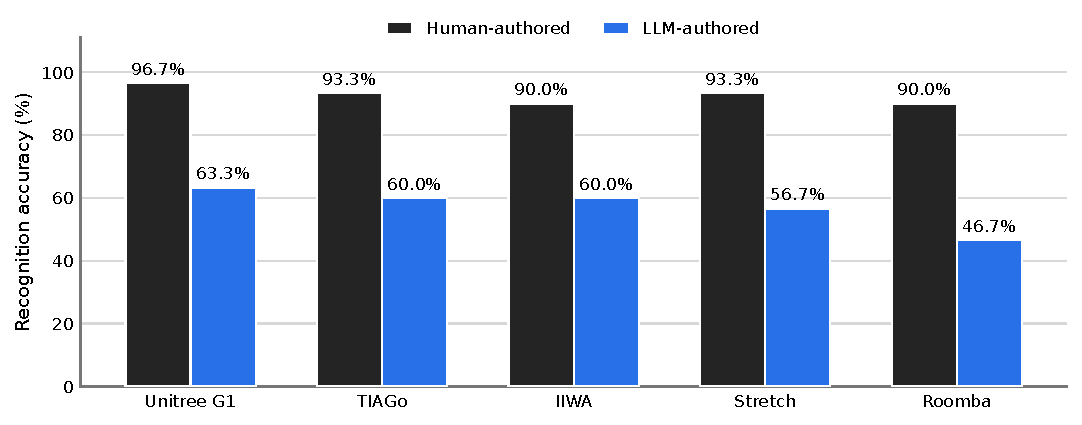
\includegraphics[width=\textwidth]{figures/figure_humanoid_attr_bars.pdf}
\caption{\textbf{[Not fixed]} Planned human recognition comparison over the a-priori feasible cues for each robot. Each group contains human-authored and LLM-authored Motion Programs plus joint-space and Cartesian-space baselines; values are provisional placeholders used only to fix the visual design. The parenthesized $n$ is the feasible count in the 90-cue inventory.}
\label{fig:humanoid-attr-bars}
\end{figure*}

\subsubsection{Failure Analysis}
We analyze failures in two steps. First, we ask whether the target body provides the indispensable carrier, i.e., whether it lies in $\mathcal{H}(B)$. A cue that requires two independently timed hands is structurally at risk on IIWA or Roomba even when its output is smooth and executable. Second, when the carrier exists, we compare the generated evidence with human GT: a failure can arise from the wrong orientation, body-relative location, movement axis or sign, timing, or coordination. Figure~\ref{fig:extension20-failure-examples} makes these distinctions concrete. Stretch preserves \texttt{fistbump\_invite} through the same arm extension, Roomba rematerializes \texttt{continue\_on\_forward\_roll} as a circular base path, and Stretch augments \texttt{visor\_search} by combining a raised arm with head scanning. In contrast, Roomba's fore--aft oscillation for \texttt{clap\_applause} cannot retain two-hand contact or bilateral symmetry; executability alone therefore does not establish recognition.

To localize errors when a human reference exists, we score program-level agreement with human GT.
Let $g_{i,a}$ and $\hat{g}_{i,a}$ denote the ground-truth and predicted body-\% coordinates on axis $a\in\{x,y,z\}$ after omitted axes are filled from the pose bank the renderer keeps.
Table~\ref{tab:humanoid-overall} reports mean absolute error
\begin{equation}
\mathrm{Loc}_a \;=\; \frac{1}{N_a}\sum_{i=1}^{N_a}\bigl|g_{i,a}-\hat{g}_{i,a}\bigr|.
\end{equation}
Reach is a six-way match on the last non-still \texttt{dir} token $d_i\in\{\mathrm{front},\mathrm{back},\mathrm{up},\mathrm{down},\mathrm{in},\mathrm{out}\}$:
\begin{equation}
\mathrm{Rch} \;=\; \frac{1}{N}\sum_{i=1}^{N}\mathbf{1}\bigl[\hat{d}_i=d_i\bigr].
\end{equation}
Palm is the same indicator on palm-normal tokens (six classes on G1).
On Tiago the gripper is only horizontal/vertical, and $0^\circ$/$180^\circ$ flips count as identical, so chance is $1/2$ rather than $1/6$.
Movement matches the GT key $(\mathrm{axis},\mathrm{sign})$ with $\mathrm{sign}\in\{+,\,-,\,{+}{-}\}$; same-axis $+$/$-$ collapse to ${+}{-}$, \texttt{path(line)} shares those keys, and \texttt{path(arc)} is scored as $(\mathrm{arc},\mathrm{plane})$:
\begin{equation}
\mathrm{Mov} \;=\; \frac{1}{N}\sum_{i=1}^{N}\mathbf{1}\bigl[\widehat{(\mathrm{axis},\mathrm{sign})}_i=(\mathrm{axis},\mathrm{sign})_i\bigr].
\end{equation}
A uniform random baseline uses $\mathbb{E}[|U-g|]$ for $U\sim\mathrm{Unif}[0,100]$ on each location axis, $\mathrm{Rch}=1/6$, $\mathrm{Plm}=1/6$ (G1) or $1/2$ (Tiago), and $\mathrm{Mov}=1/9$ over axis$\times$sign.

\subsubsection{Automatic Structural Audit}
The automatic audit measures coverage and program structure rather than recognition. Among the 20 added cues, the a-priori feasible subsets contain 8 IIWA, 12 Stretch, and 5 Roomba cues. Relative to the original 30-cue screen, this expands each feasible inventory from 15 to 23 cues on IIWA ($+53.3\%$), 16 to 28 on Stretch ($+75.0\%$), and 12 to 17 on Roomba ($+41.7\%$). We then assign each generated program a deterministic structural label from its required carrier, feasibility prior, and used carriers: \emph{preserved}, \emph{carrier-transferred}, \emph{rematerialized}, \emph{augmented}, or \emph{at-risk substitute}. Figure~\ref{fig:extension20-structural-audit} shows that IIWA mainly preserves feasible one-arm cues, Stretch often recruits an additional head or torso channel, and Roomba rematerializes only five selected cues under the strict prior. The remaining cases are retained in the human-evaluation deck as deliberately difficult probes, not counted as automatic successes.

\begin{figure*}[t]
\centering
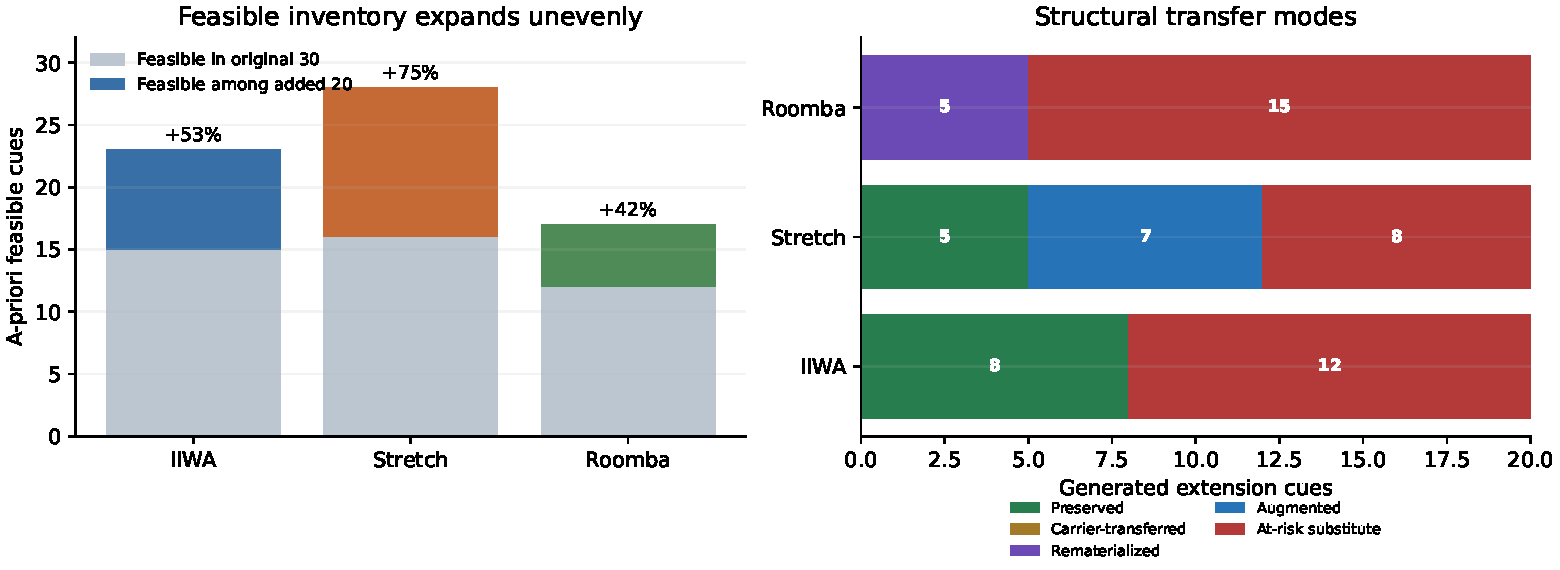
\includegraphics[width=\textwidth]{figures/figure_extension20_structural_audit.pdf}
\caption{Automatic structural audit of the 20-cue extension. Left: feasible cue counts before and after adding the selected cues; percentages report growth relative to each robot's feasible count in the original 30-cue screen. Right: deterministic structural labels for all 20 generated programs per robot. \emph{At-risk substitute} means that the a-priori carrier requirement is unavailable; it is not a human-recognition judgment.}
\label{fig:extension20-structural-audit}
\end{figure*}



\section{Results}
\label{sec:analysis}
\label{sec:nonhumanoid}
We organize the results around two questions, one for bodies that have human-like carriers and one for bodies that lack them.
Figure~\ref{fig:humanoid-attr-bars} is not yet a completed five-robot result; only the existing G1 and Tiago screens are empirical recognition summaries.
For the other bodies, we report the planned feasible denominator, the program-level diagnostics in Table~\ref{tab:humanoid-overall}, and qualitative evidence in Figs.~\ref{fig:offtheshelf}, \ref{fig:physical-difficulty-grid}, and~\ref{fig:extension20-failure-examples} without converting executability into a recognition claim.

\begin{figure*}[!t]
\centering
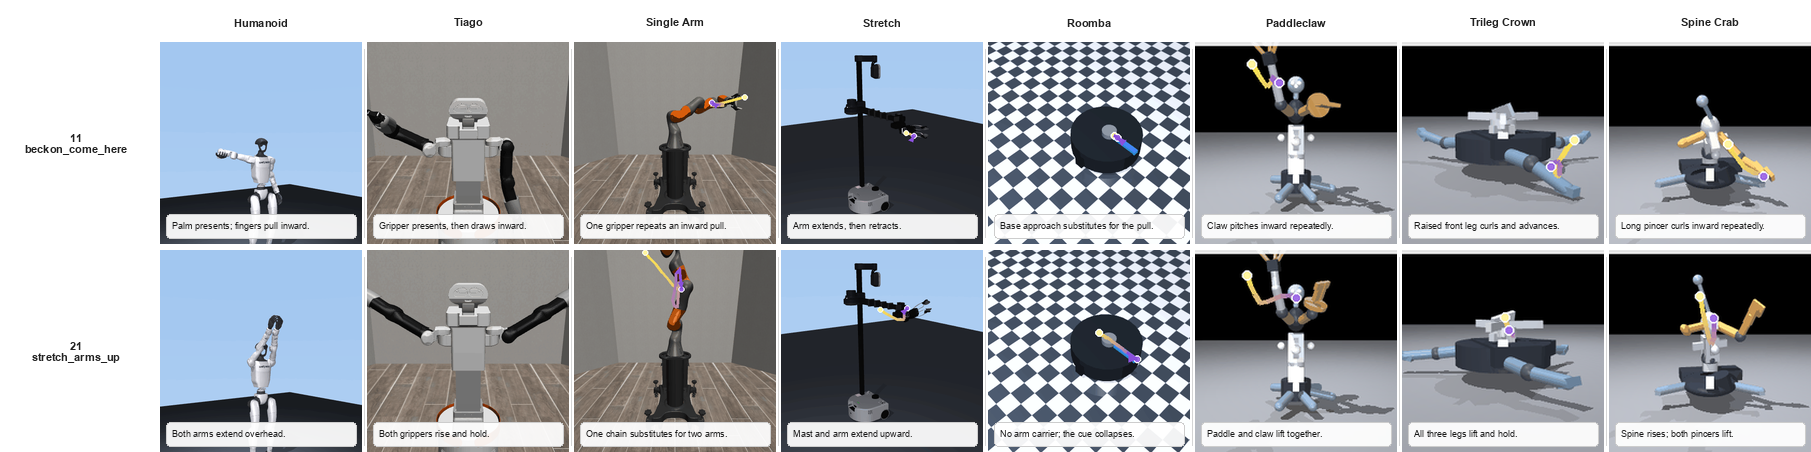
\includegraphics[width=\textwidth]{figures/figure_physical_difficulty_grid.png}
\caption{The same two cues rendered on all eight embodiments. Each row fixes the intended cue, exposing how its evidence is retained, rematerialized onto another carrier, or lost as available channels change. Colored traces show carrier trajectories for the six non-Humanoid/Tiago bodies. The first five columns use Gemini-authored Motion Programs for catalog robots; the last three are synthetic morphologies.}
\label{fig:physical-difficulty-grid}
\end{figure*}

\begin{figure*}[t]
\centering
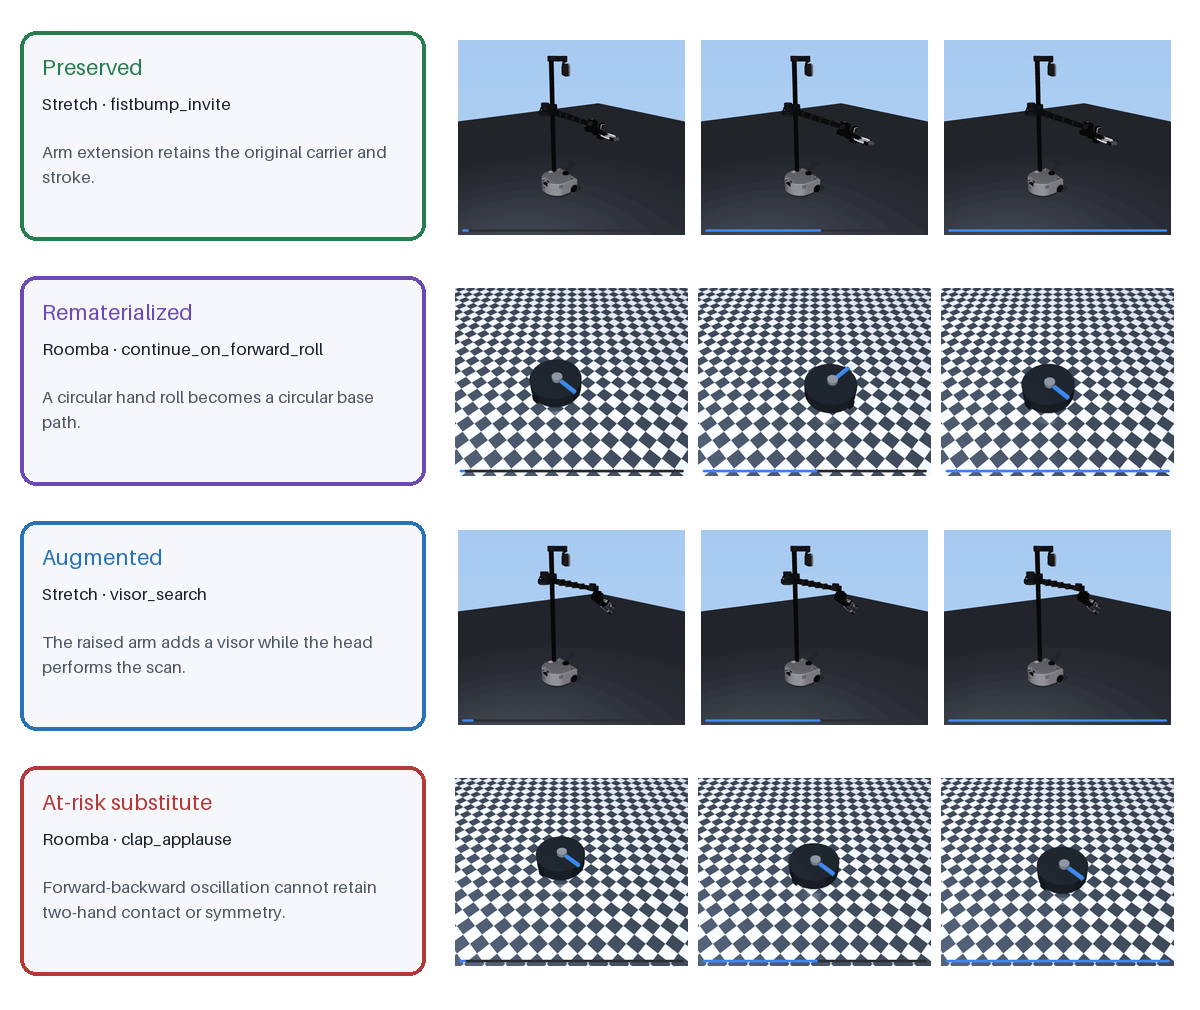
\includegraphics[width=\textwidth]{figures/figure_extension20_failure_examples.png}
\caption{Four concrete outcomes in the 20-cue extension, shown at the beginning, middle, and end of each clip. Preservation keeps the original carrier and stroke; rematerialization reconstructs the motion on a different body; augmentation adds a second evidential channel. An at-risk substitute remains executable but omits indispensable structure, as in Roomba \texttt{clap\_applause}. These labels motivate, but do not replace, hard-negative human recognition.}
\label{fig:extension20-failure-examples}
\end{figure*}

\subsection{Human-like Bodies (G1, Tiago): Which Attributes Does Authoring Miss?}
\label{sec:results-humanlike}
G1 and Tiago provide the carriers a human gesture needs, so any remaining gap reflects what automatic authoring misses rather than what the body lacks.

\paragraph{Unitree G1}
On the current 30-cue screen, human-authored and LLM-authored Motion Programs reach $96.7\%$ and $63.3\%$, respectively.
The harder 90-cue G1 pilot yields $43/79$ answered 4AFC trials ($54.4\%$, chance $25\%$), so the automatic programs retain identity above close form and meaning alternatives but remain well below the human reference.
Table~\ref{tab:humanoid-overall} localizes the gap: Reach, Palm, and Movement agreement are $47.2\%$, $48.6\%$, and $50.6\%$, while the two-arm group drops to $19.0\%$ Movement.
A misplaced and forward-facing \texttt{salute} becomes a generic raised hand; \texttt{beckon\_come\_here} may lose its repeated inward flap; and \texttt{draw\_circle\_repeat} can preserve circularity in the wrong plane.
Conversely, the G1 \texttt{beckon} sequence in Fig.~\ref{fig:critical-attributes} succeeds because palm facing, hand location, and repeated inward movement agree.

\paragraph{Tiago}
The current 30-cue screen gives $93.3\%$ for human-authored programs and $60.0\%$ for LLM-authored programs.
Thus replacing articulated palms with H/V grippers does not erase the vocabulary, but automatic authoring retains the same substantial gap seen on G1.
Table~\ref{tab:humanoid-overall} reports $49.1\%$ Reach, $52.8\%$ Palm, and $56.1\%$ Movement agreement.
Movement is strongest for one-arm cues ($74.2\%$) and weakest when two coordinated arms are required ($16.7\%$).
The Tiago \texttt{depict\_flying\_bird} in Fig.~\ref{fig:offtheshelf} preserves bilateral span and repeated flapping, whereas a gripper-only raise cannot reliably preserve the palm contrast among \texttt{stop}, \texttt{highfive}, and \texttt{salute}.

\paragraph{Interpretation}
On both bodies the model has access to every carrier it needs, yet it places, orients, and strokes them incorrectly, and fails most where two arms must be coordinated. The generated program resembles the human gesture in outline but omits the attribute that separates it from its neighbours---the signature of imitation without understanding.

\subsection{Constrained and Unfamiliar Bodies (IIWA, Stretch, Roomba): Which Meanings Survive?}
\label{sec:results-constrained}
On IIWA, Stretch, and Roomba the human carrier is partly or entirely missing from $\mathcal{H}(B)$, so the question shifts from which attributes are missed to which meanings survive preservation, carrier transfer, or rematerialization. The three synthetic morphologies extend the same question to bodies with no catalog counterpart.

\paragraph{Single arm (IIWA)}
The planned study evaluates the $47/90$ feasible cues; its recognition rate is not fixed, and the Single Arm bars in Fig.~\ref{fig:humanoid-attr-bars} are placeholders.
This denominator excludes cues whose identity indispensably requires face contact, fine digits, or two independent hands.
On the generated 30-cue feasible intersection ($n{=}15$), Table~\ref{tab:humanoid-overall} gives $80.0\%$ Reach, $71.4\%$ H/V Palm, and $73.3\%$ Movement agreement.
Figure~\ref{fig:physical-difficulty-grid} shows both preservation and loss under carrier reduction: the single gripper retains the repeated inward pull of \texttt{beckon\_come\_here}, whereas \texttt{stretch\_arms\_up} can preserve only the upward extension, not the bilateral arm configuration.
These are physical omissions, not merely axis errors.

\paragraph{Stretch}
Stretch contributes $53/90$ feasible cues to the planned study, but its recognition rate is not yet fixed.
The evaluation is intentionally restricted to $x$, $z$, Reach, and Movement because lateral placement and an independent palm are not stable communicative channels on this platform.
For its generated 30-cue feasible intersection ($n{=}16$), Table~\ref{tab:humanoid-overall} reports $91.7\%$ Reach and $81.2\%$ Movement, with $13.9$ and $6.2$ body-\% error on $x$ and $z$.
In Fig.~\ref{fig:physical-difficulty-grid}, Stretch rematerializes \texttt{beckon\_come\_here} as extension followed by retraction and renders \texttt{stretch\_arms\_up} through mast and arm elevation.
The gross direction remains legible, but palm articulation and bilateral symmetry are unavailable.

\paragraph{Roomba}
Only $33/90$ cues satisfy the a-priori feasibility rule, and no fixed recognition rate is yet available.
This is the strongest test of whether a cue can survive as movement alone rather than as a hand pose at a body-relative location.
Movement agreement is $83.3\%$ on the 12 feasible generated screening cues in Table~\ref{tab:humanoid-overall}.
In Fig.~\ref{fig:physical-difficulty-grid}, Roomba can reinterpret the inward pull of \texttt{beckon\_come\_here} as base approach, but \texttt{stretch\_arms\_up} loses its defining carrier and collapses to an underspecified base motion.
Likewise, \texttt{stop\_palm\_out} and \texttt{highfive\_invite} can both collapse to advance-and-hold once palm and hand location disappear (Fig.~\ref{fig:teaser}b).
The $720^\circ$ spin used for \texttt{raise\_fists\_victory} in Fig.~\ref{fig:offtheshelf} is expressive, but without perceptual validation it signals generic excitement rather than victory specifically.

\paragraph{Synthetic morphologies}
Paddleclaw, Trileg Crown, and Spine Crab retain $84$, $55$, and $75$ feasible cues, respectively, but have no fixed recognition rates.
They therefore test compilation and aliasing on unseen bodies, not superiority over the catalog platforms; Table~\ref{tab:humanoid-overall} omits them until comparable human-authored attribute references are fixed.
Figure~\ref{fig:physical-difficulty-grid} holds cue identity fixed across the three new morphologies.
For \texttt{beckon\_come\_here}, Paddleclaw repeatedly pitches its claw, Trileg Crown curls a raised front leg while advancing, and Spine Crab curls its long pincer; for \texttt{stretch\_arms\_up}, they lift two branches, all three legs, and the spine-plus-pincer pair, respectively.
The outputs preserve movement structure while changing the physical carrier, although none reproduces a human palm exactly.
Across all three, the key failure is contrast collapse: a motion may be plausible and executable while multiple intended cues share the same remaining carrier and stroke.

\paragraph{Interpretation}
Off the human body, what survives is predominantly movement structure---axis, repetition, approach---whereas cues distinguished by palm orientation or body-relative location collapse onto the same remaining stroke. Because people read meaning through unfamiliar carriers, this collapse is better explained by a generator that does not know how to recruit the remaining carriers to keep cues apart than by a ceiling on what observers can read; the planned constrained-body recognition study is required to confirm it.

\section{Conclusion}
Embodied agents are expressive whether or not they were designed to be.
People read intent in moving shapes, animal displays, and prosthetic limbs, so a robot's motion will be interpreted regardless of its body; what varies is whether that body, as used by its generator, preserves the evidence for the intended meaning.
Orientation, body-relative location, and movement provide compact handles for posing that question, complemented by timing, repetition, scale, coordination, and context.

Our results are evidence about generation rather than a benchmark score.
On human-like bodies, every necessary carrier is available, yet LLM-authored programs are recognized at $63.3\%$ and $60.0\%$ against $96.7\%$ and $93.3\%$ for human authors, because they misplace, misorient, or mistime those carriers: they imitate a gesture's outline without understanding which attribute carries its meaning.
On non-humanoid bodies, generation draws from a narrower repertoire: some cues transfer or rematerialize, while others collapse together once their defining evidence has no human form left to copy.

Motion Programs are a stopgap for this situation.
They let people and LLMs author the same attribute-level evidence and compile it through morphology-specific renderers, which makes today's gestures possible and today's failures legible; but the understanding of the body still resides in the schema and the human authors, not in the model.

This leaves two concrete problems for the community.
First, how can we lower the authoring barrier so that every robot can be given an editable repertoire of recognizable gestures, even when humans must still define the semantics?
Second, and more fundamentally, how can models learn to reason about their own morphology well enough to invent the right carrier and motion, rather than merely imitate the surface form of a human gesture?
Answering the second question will require evaluation on meaning recognition across genuinely different bodies, not only realism on a familiar human skeleton---and it is the step that would let every embodied agent express meaning with the body it actually has.

\appendix

\section{50-Cue Evaluation Inventory}
\label{app:cue-inventory}
\begin{table}[t]
\centering
\scriptsize
\setlength{\tabcolsep}{3pt}
\renewcommand{\arraystretch}{1.05}
\begin{tabularx}{\columnwidth}{@{}r>{\raggedright\arraybackslash}X>{\raggedright\arraybackslash}p{2.3cm}@{}}
\toprule
\textbf{ID} & \textbf{Cue} & \textbf{A-priori feasible morphologies} \\
\midrule
1 & \texttt{nod\_yes} & G1, TIAGo, IIWA, Stretch, Roomba \\
2 & \texttt{shake\_head\_no} & G1, TIAGo, IIWA, Stretch, Roomba \\
4 & \texttt{gaze\_shift\_avoid} & G1, TIAGo, IIWA, Stretch, Roomba \\
6 & \texttt{tilt\_head\_curious} & G1, TIAGo, IIWA, Stretch, Roomba \\
\bottomrule
\end{tabularx}
\caption{Head / torso cues in the 50-cue evaluation inventory ($n=4$). Feasibility follows the carrier-preservation rule in Sec.~\ref{sec:experiment} and does not imply recognition.}
\label{tab:cue-inventory-50-1}
\end{table}

\begin{table}[t]
\centering
\scriptsize
\setlength{\tabcolsep}{3pt}
\renewcommand{\arraystretch}{1.05}
\begin{tabularx}{\columnwidth}{@{}r>{\raggedright\arraybackslash}X>{\raggedright\arraybackslash}p{2.3cm}@{}}
\toprule
\textbf{ID} & \textbf{Cue} & \textbf{A-priori feasible morphologies} \\
\midrule
7 & \texttt{cover\_yawn\_sleepy} & G1, TIAGo \\
8 & \texttt{rub\_eye\_tired} & G1, TIAGo \\
10 & \texttt{point\_self} & G1, TIAGo, Stretch \\
13 & \texttt{salute} & G1, TIAGo \\
25 & \texttt{facepalm} & G1, TIAGo \\
31 & \texttt{self\_scratch\_head\_confused} & G1, TIAGo \\
32 & \texttt{pat\_stomach} & G1, TIAGo, Stretch \\
33 & \texttt{fan\_face\_hot} & G1, TIAGo \\
37 & \texttt{cover\_mouth\_gasp} & G1, TIAGo \\
42 & \texttt{throat\_cut\_stop} & G1, TIAGo, Stretch \\
43 & \texttt{visor\_search} & G1, TIAGo, Stretch \\
\bottomrule
\end{tabularx}
\caption{Head / torso + one arm cues in the 50-cue evaluation inventory ($n=11$). Feasibility follows the carrier-preservation rule in Sec.~\ref{sec:experiment} and does not imply recognition.}
\label{tab:cue-inventory-50-2}
\end{table}

\begin{table}[t]
\centering
\scriptsize
\setlength{\tabcolsep}{3pt}
\renewcommand{\arraystretch}{1.05}
\begin{tabularx}{\columnwidth}{@{}r>{\raggedright\arraybackslash}X>{\raggedright\arraybackslash}p{2.3cm}@{}}
\toprule
\textbf{ID} & \textbf{Cue} & \textbf{A-priori feasible morphologies} \\
\midrule
3 & \texttt{draw\_circle\_repeat} & G1, TIAGo, IIWA, Stretch, Roomba \\
5 & \texttt{fist\_pump} & G1, TIAGo, IIWA, Stretch, Roomba \\
9 & \texttt{point\_you} & G1, TIAGo, IIWA, Stretch \\
11 & \texttt{beckon\_come\_here} & G1, TIAGo, IIWA, Stretch, Roomba \\
12 & \texttt{stop\_palm\_out} & G1, TIAGo, IIWA, Stretch \\
14 & \texttt{raise\_index\_one\_moment} & G1, TIAGo \\
15 & \texttt{highfive\_invite} & G1, TIAGo, IIWA, Stretch \\
17 & \texttt{flex\_bicep} & G1, TIAGo \\
26 & \texttt{depict\_tree} & G1, TIAGo, IIWA, Stretch, Roomba \\
29 & \texttt{depict\_small\_object} & G1, TIAGo, IIWA, Stretch, Roomba \\
40 & \texttt{fistbump\_invite} & G1, TIAGo, IIWA, Stretch \\
44 & \texttt{yield\_turn} & G1, TIAGo, IIWA, Stretch, Roomba \\
45 & \texttt{request\_turn} & G1, TIAGo, IIWA, Stretch \\
48 & \texttt{slow\_down\_request\_palm\_down} & G1, TIAGo, IIWA, Stretch \\
61 & \texttt{clarification\_request\_palm\_tilt} & G1, TIAGo, IIWA, Stretch \\
65 & \texttt{continue\_on\_forward\_roll} & G1, TIAGo, IIWA, Stretch, Roomba \\
69 & \texttt{interrupt\_hard} & G1, TIAGo, IIWA, Stretch, Roomba \\
70 & \texttt{interrupt\_soft} & G1, TIAGo, IIWA, Stretch, Roomba \\
81 & \texttt{wait\_for\_me\_backward\_palm} & G1, TIAGo, Stretch \\
83 & \texttt{frustration\_down\_throw} & G1, TIAGo \\
\bottomrule
\end{tabularx}
\caption{One arm / hand cues in the 50-cue evaluation inventory ($n=20$). Feasibility follows the carrier-preservation rule in Sec.~\ref{sec:experiment} and does not imply recognition.}
\label{tab:cue-inventory-50-3}
\end{table}

\begin{table}[t]
\centering
\scriptsize
\setlength{\tabcolsep}{3pt}
\renewcommand{\arraystretch}{1.05}
\begin{tabularx}{\columnwidth}{@{}r>{\raggedright\arraybackslash}X>{\raggedright\arraybackslash}p{2.3cm}@{}}
\toprule
\textbf{ID} & \textbf{Cue} & \textbf{A-priori feasible morphologies} \\
\midrule
16 & \texttt{shrug\_idk} & G1, TIAGo \\
18 & \texttt{air\_quotes} & G1, TIAGo \\
19 & \texttt{arms\_open\_welcome} & G1, TIAGo \\
20 & \texttt{hands\_up\_surrender} & G1, TIAGo \\
21 & \texttt{stretch\_arms\_up} & G1, TIAGo \\
22 & \texttt{raise\_fists\_victory} & G1, TIAGo \\
23 & \texttt{cross\_arms\_defensive} & G1, TIAGo \\
24 & \texttt{palms\_together\_thank\_you} & G1, TIAGo \\
27 & \texttt{depict\_big\_bowl} & G1, TIAGo, IIWA, Stretch, Roomba \\
28 & \texttt{depict\_lion} & G1, TIAGo, IIWA, Stretch, Roomba \\
30 & \texttt{depict\_flying\_bird} & G1, TIAGo, IIWA, Stretch, Roomba \\
51 & \texttt{scale\_expand} & G1, TIAGo, Roomba \\
71 & \texttt{self\_hug} & G1, TIAGo \\
78 & \texttt{push\_pull\_dual} & G1, TIAGo \\
90 & \texttt{clap\_applause} & G1, TIAGo \\
\bottomrule
\end{tabularx}
\caption{Two arms / hands cues in the 50-cue evaluation inventory ($n=15$). Feasibility follows the carrier-preservation rule in Sec.~\ref{sec:experiment} and does not imply recognition.}
\label{tab:cue-inventory-50-4}
\end{table}


{\scriptsize
\bibliographystyle{IEEEtran}
\bibliography{main,root2_additions}
}


\end{document}
